\chapter{Experimental Results}
\label{chap:\currfilebase}
...

\begin{figure}[!ht]
    \centering
    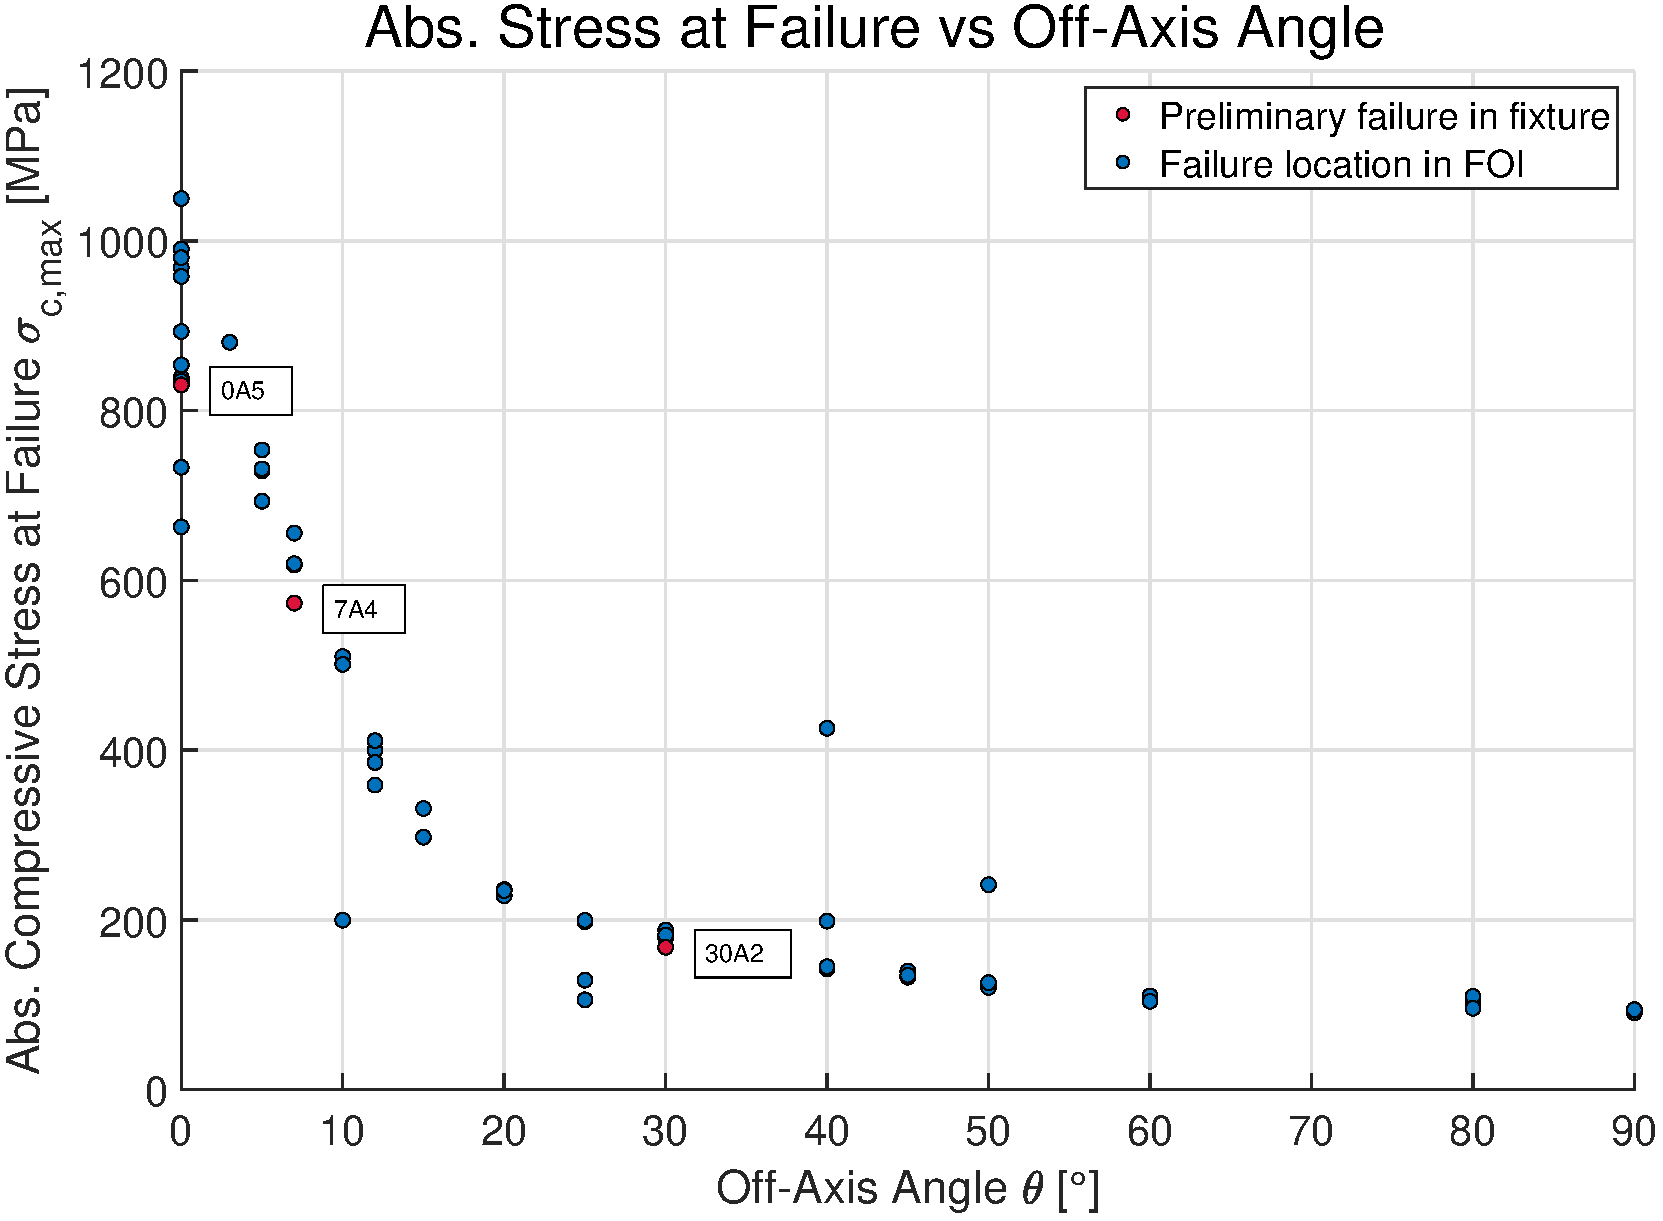
\includegraphics[scale=0.4]{\imgpath/\currfilebase/Strength_OffAngle_1.pdf}
    \caption{Abs. compressive stress at failure over off axis angle, all measurements}
    \label{fig:strength_offAngle_1}
\end{figure}
\begin{figure}[!ht]
    \centering
    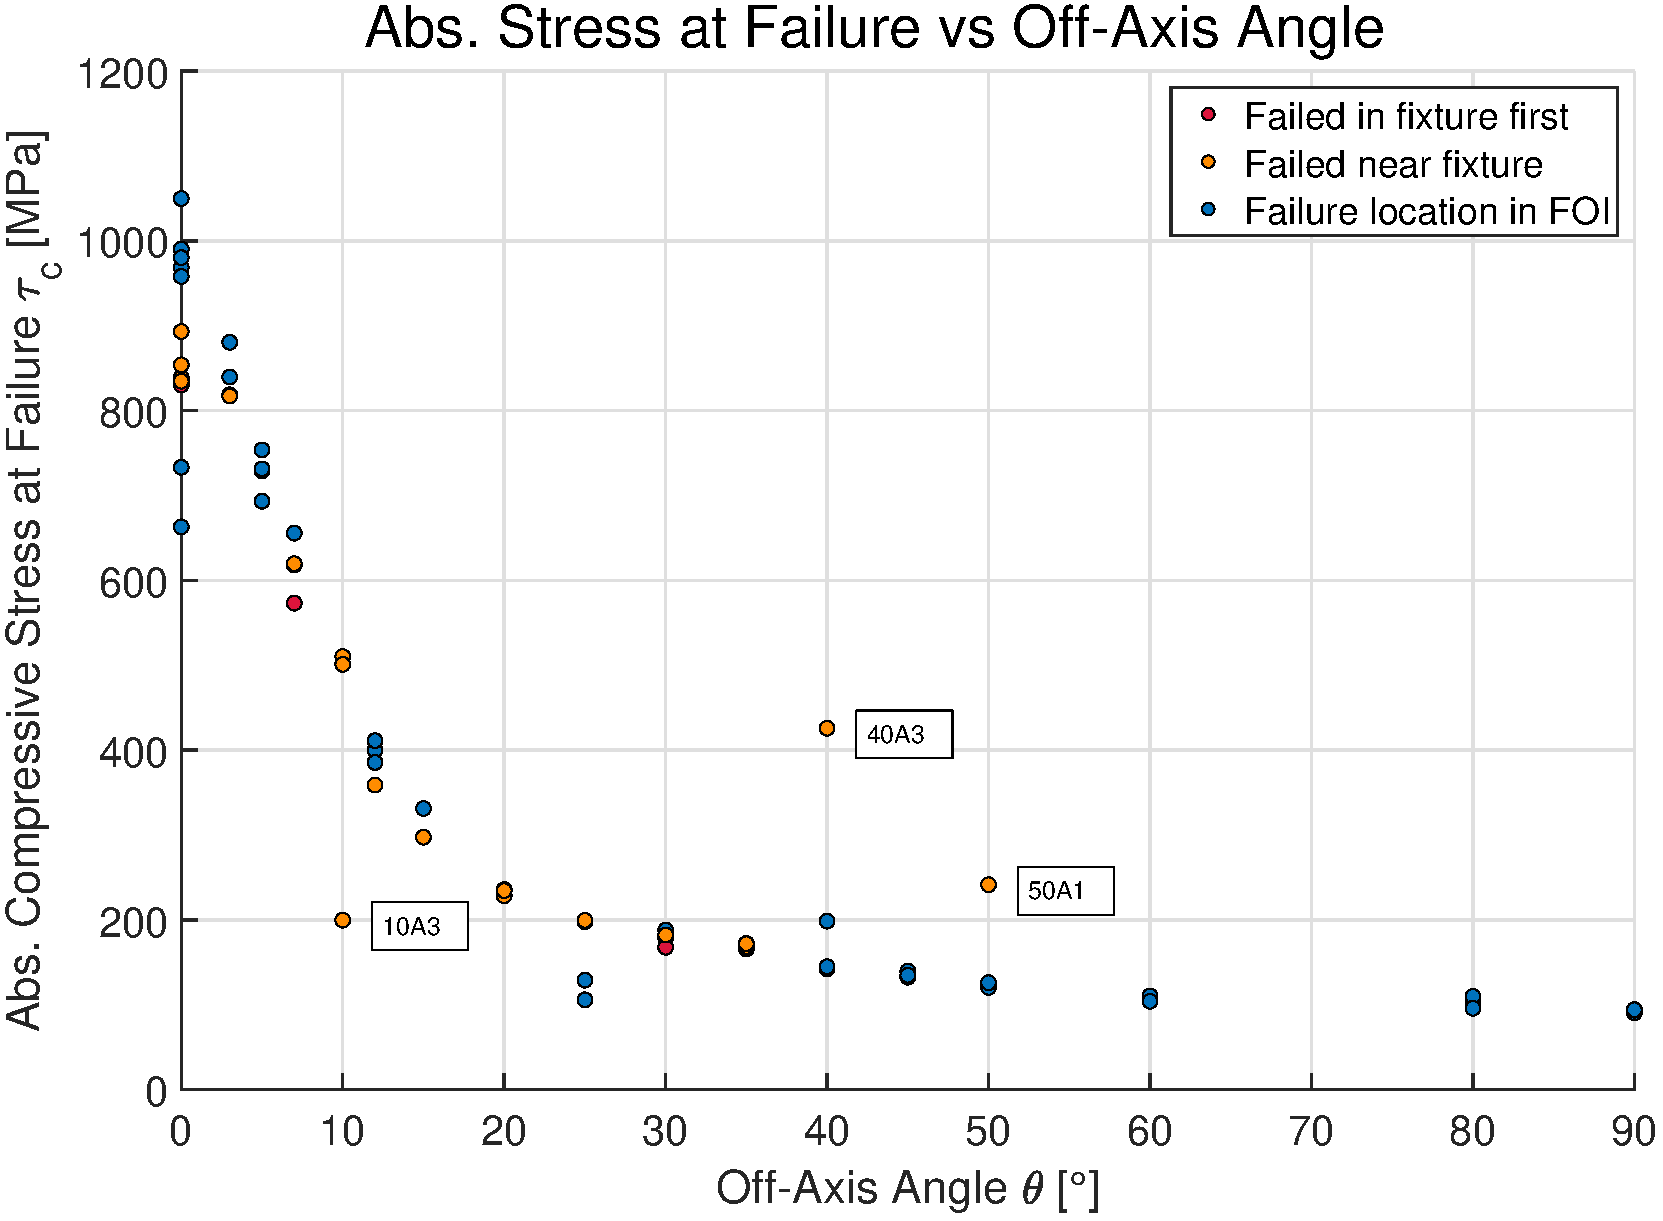
\includegraphics[scale=0.4]{\imgpath/\currfilebase/Strength_OffAngle_2.pdf}
    \caption{Abs. compressive stress at failure over off axis angle, \#2}
    \label{fig:strength_offAngle_2}
\end{figure}
\begin{figure}[!ht]
    \centering
    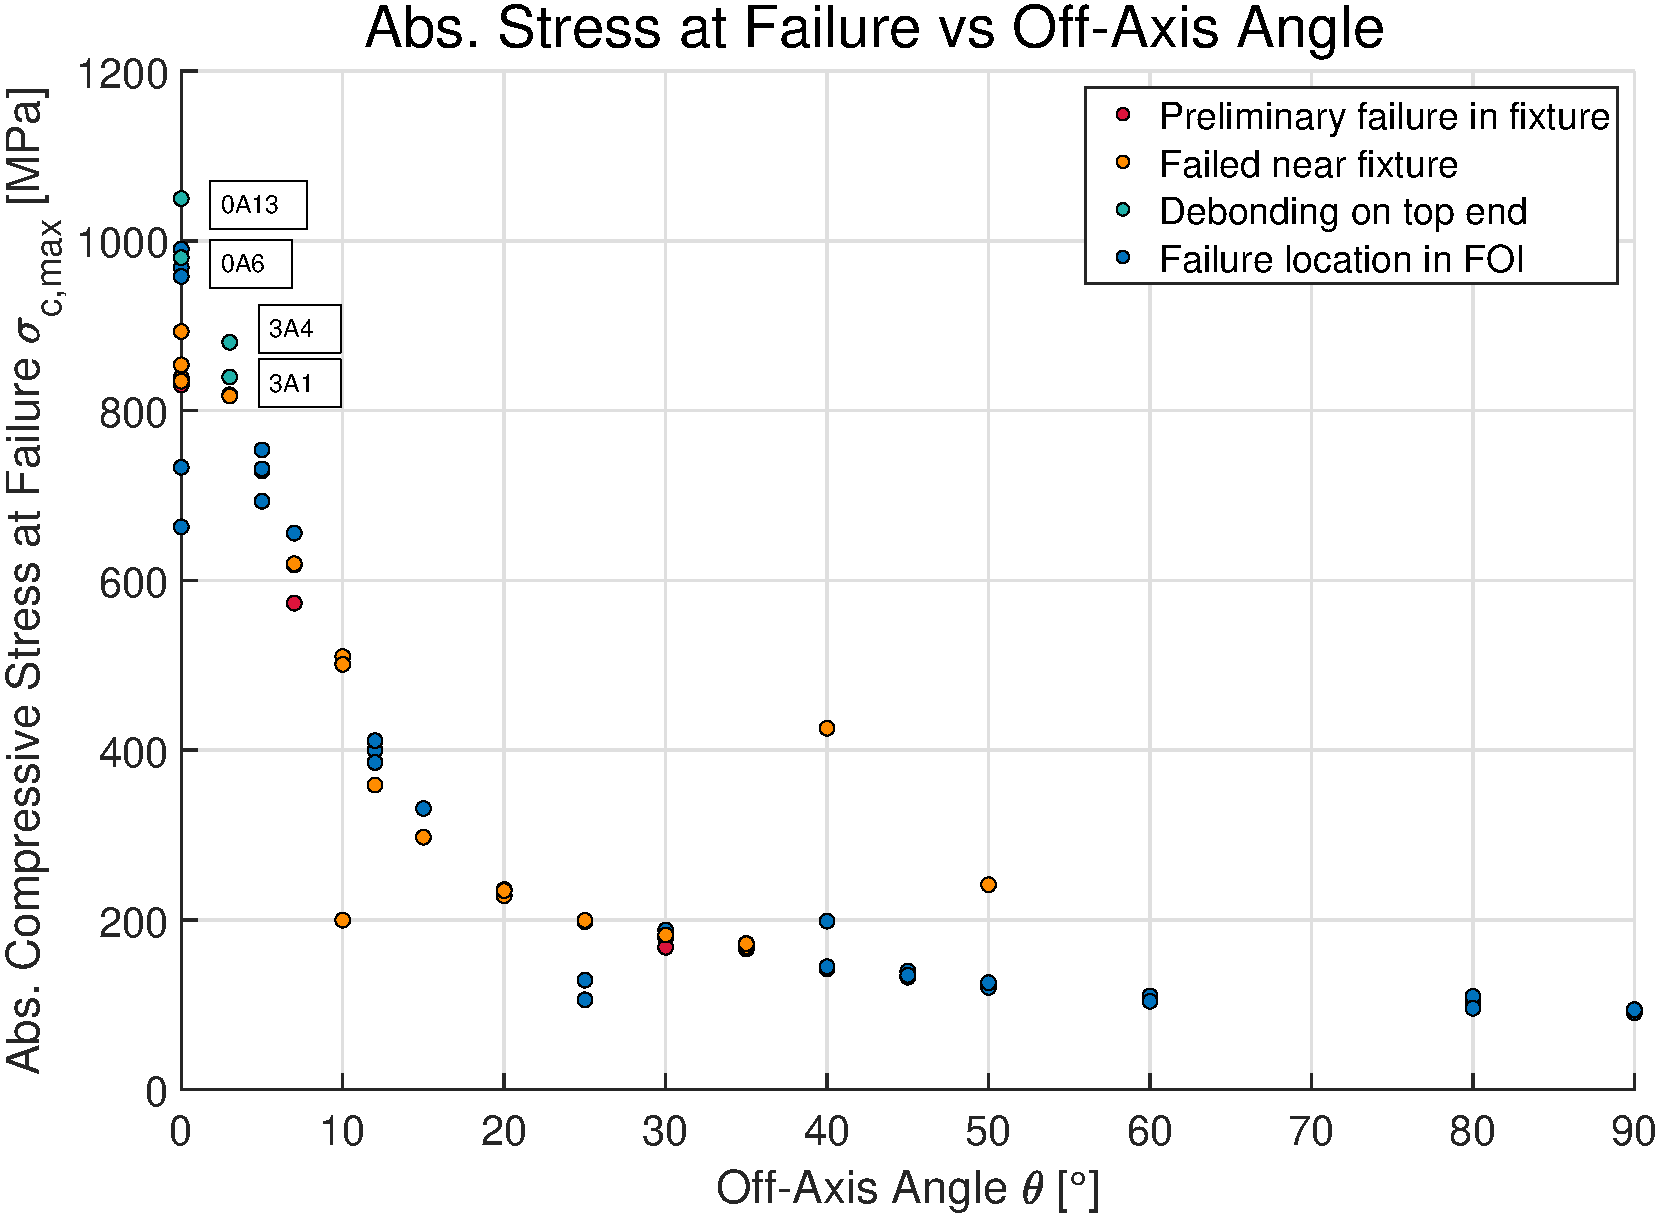
\includegraphics[scale=0.4]{\imgpath/\currfilebase/Strength_OffAngle_3.pdf}
    \caption{Abs. compressive stress at failure over off axis angle, \#3}
    \label{fig:strength_offAngle_3}
\end{figure}
\begin{figure}[!ht]
    \centering
    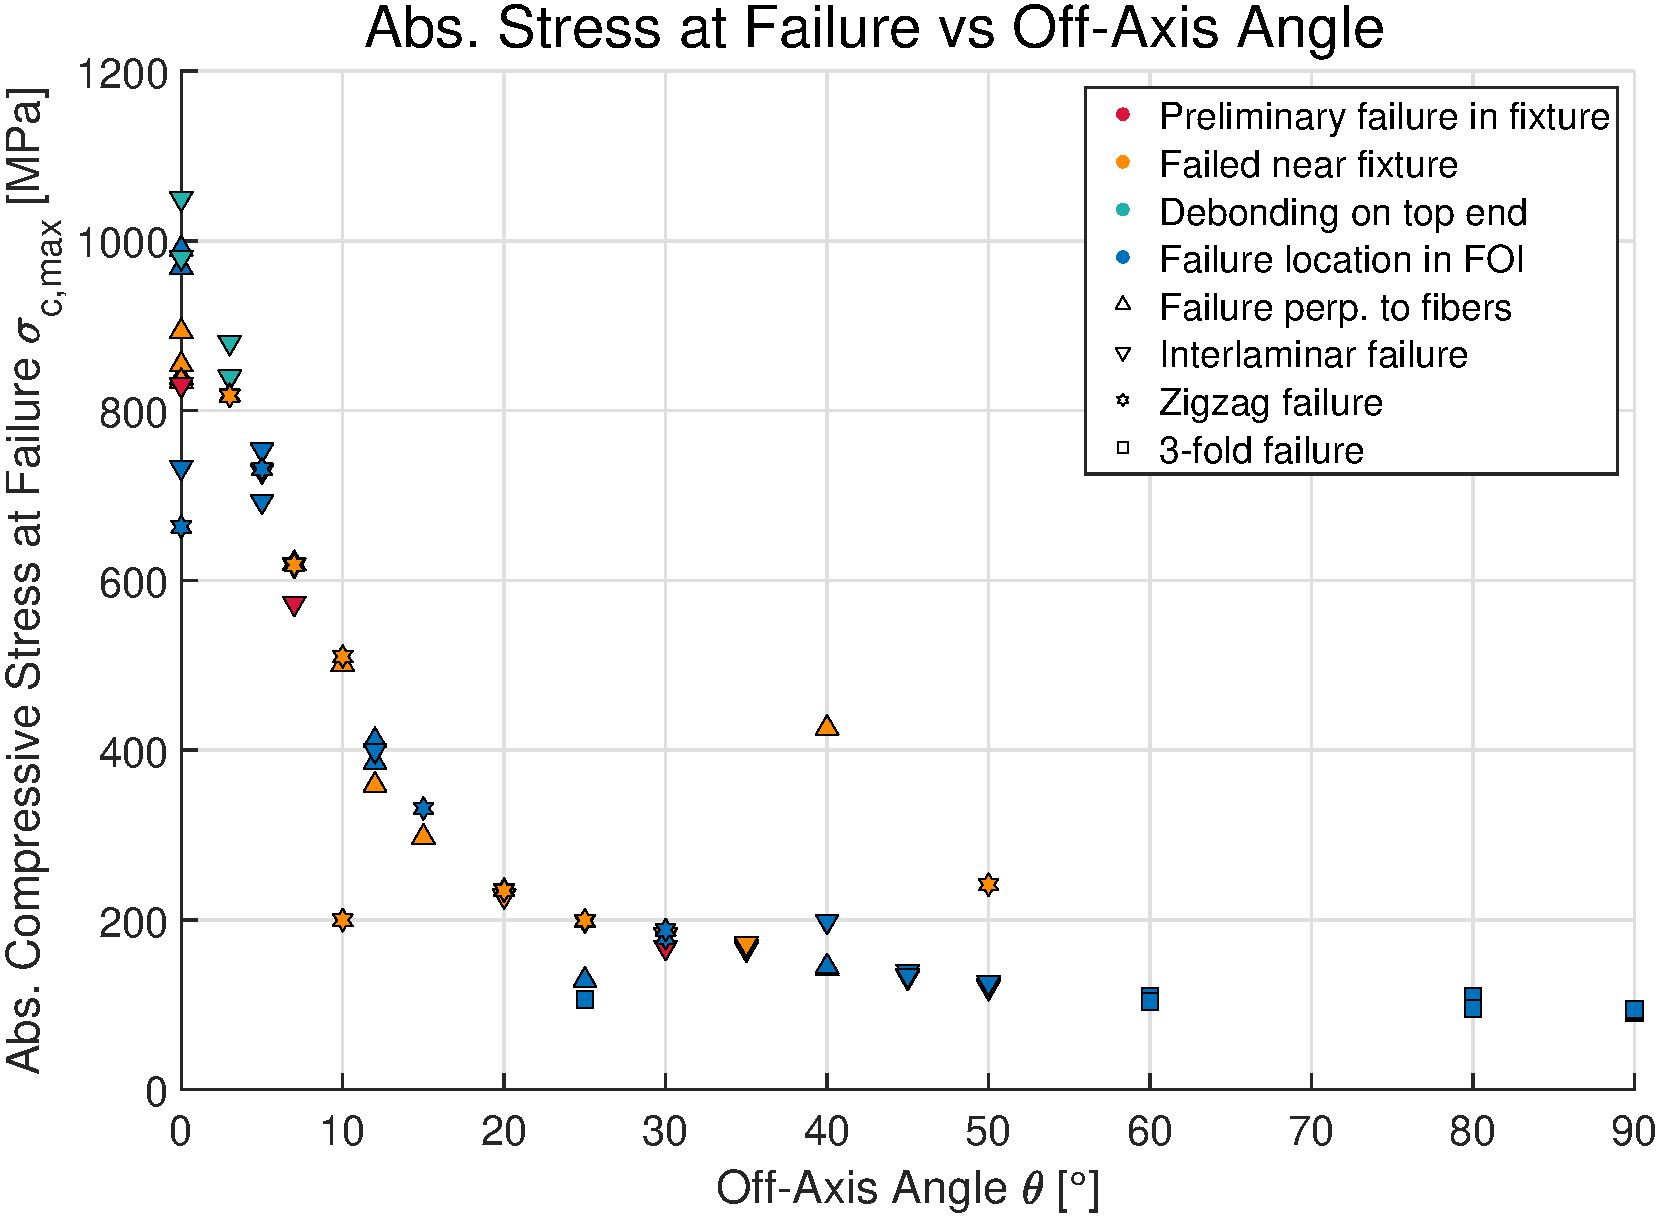
\includegraphics[scale=0.4]{\imgpath/\currfilebase/Strength_OffAngle_4.pdf}
    \caption{Abs. compressive stress at failure over off axis angle, \#4}
    \label{fig:strength_offAngle_4}
\end{figure}
\begin{figure}[!ht]
    \centering
    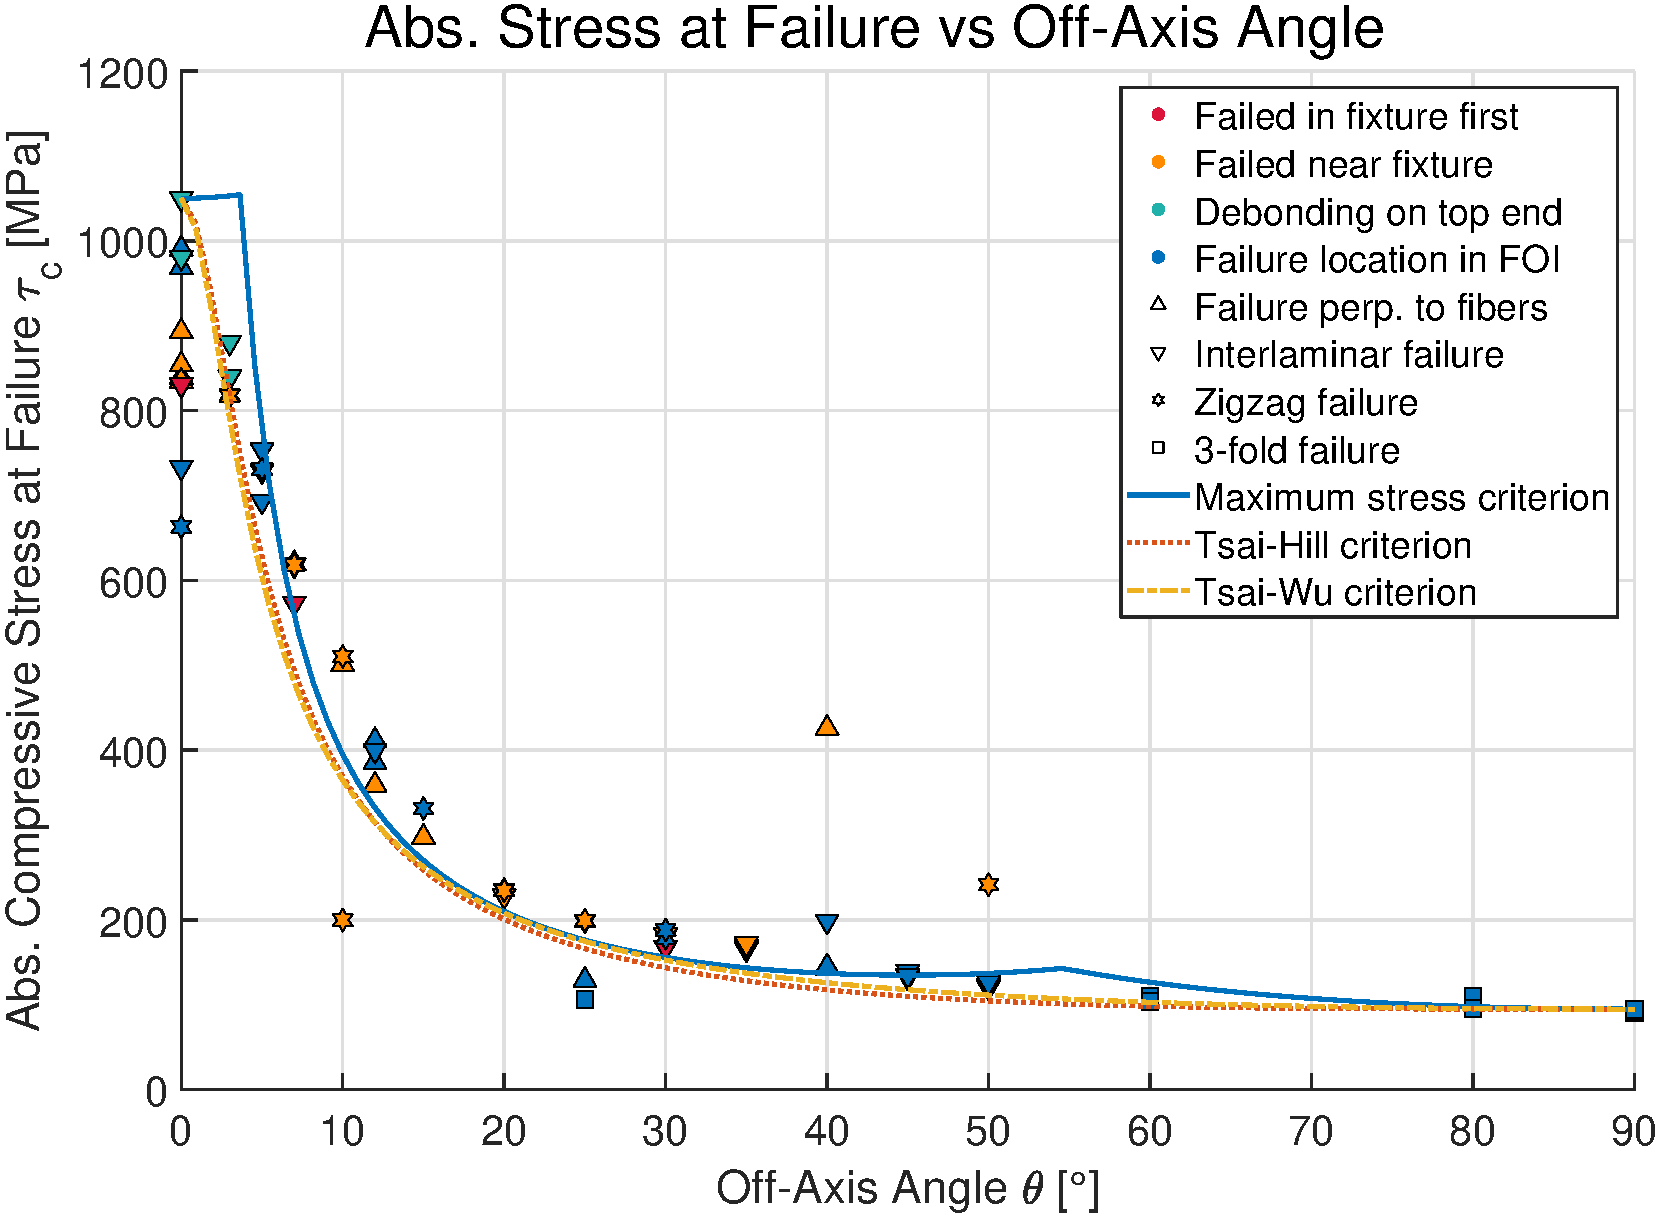
\includegraphics[scale=0.4]{\imgpath/\currfilebase/Strength_OffAngle_5.pdf}
    \caption{Abs. compressive stress at failure over off axis angle, \#5}
    \label{fig:strength_offAngle_5}
\end{figure}
% The following measurement results are represented as the positioning error motions of the different target point over time, the relevant temperature over time and a surface plot of the positioning error motions relative to the first positioning error motion over time and target point position. Where the later aims to show the deviations neglecting their geometrical error contribution.\par
% Straightness error motions are not addressed since their deviations lie within the measurement uncertainty of the position measuring instrument.\par
% All measurement results shown in this thesis are conducted using the measurement head of the linear encoder itself (Figure~{\ref{fig:heidenhainvm182_3d}}). Measurement results using another scanning head are left out as they cannot be compared with the ones listed. 
% Additional measurement results can be found in the appendix.
% \newpage

% \section{Cold test\label{sec:resultcold}}

% %appendix: cold test 17112017 n_t=140

% \subsection*{Observations in a cold test over three days}
% In Figure~{\ref{fig:coldtest_24112017_devtemp}} the positioning error motion of the individual target points and different temperatures of importance are depicted over time. The positioning error motions of the individual target points show a similar curvature with respect to each other but have different initial values. All temperature curvatures follow the same pattern but with different magnitudes of the deflections. One may notice the contemporaneous deflections of the negative positioning error motion and environmental temperature especially at temperature peaks. When considering the relative positioning error motion as depicted in Figure~{\ref{fig:coldtest_24112017_surf}}, it becomes apparent that the time dependant deviation range remains below {\SI{3}{\micro\metre}} for all target points alike.
% \newpage

% \begin{figure}[H]
% \centering
% \includegraphics[width=0.85\linewidth]{figures/measurementresults/cold/coldtest_24112017_devtemp}
% \caption[Positioning error motions motions and relevant temperatures cold 24.11.2017]{Positioning error motions and relevant temperature profiles over time of the cold test started on November 24th 2017. Setting parameter $n_t=140$}
% \label{fig:coldtest_24112017_devtemp}
% \end{figure}
% \vspace{2\baselineskip}
% \begin{figure}[H]
% \centering
% \includegraphics[width=0.85\linewidth]{figures/measurementresults/cold/coldtest_24112017_surf}
% \caption[Relative positioning error motion cold 24.11.2017]{Relative positioning error motion of the cold test started on November 24th 2017. Setting parameter $n_t=140$}
% \label{fig:coldtest_24112017_surf}
% \end{figure}
% %---
% \newpage

% %----------------------------------------------------------------------
% \section{Warm-Cold test\label{sec:resultwarmcold}}

% %appendix: warmcoldtest 07112017 v_w=5000
% %appendix: warmcoldtest 10112017 v_w=12500 special test

% \subsection*{Observations in a warm-cold test with an oscillation feed rate of 12500 mm/min}
% As previously seen in a cold test (Section~{\ref{sec:resultcold}}) the positioning error motions over time of the different target point show a similar pattern with respect to each other but start at increasing initial values (Figure~{\ref{fig:warmcoldtest_11112017a_devtemp}}). A distinct effect that can be observed in a warm-cold test is the rise in the temperatures of the Y-axis spindle motor and the spindle nut during the first phase of the test. Those temperatures both rise until a saturation temperature is reached in the warm phase and approximate the the environmental temperature in the cold phase while relating to lead-lag properties. Especially when considering the relative positioning error in Figure~{\ref{fig:warmcoldtest_11112017a_surf}} the very same lead-lag properties may be identified in the negative of the deviations. The range of the relative positioning error motions over time remains similar compared to a cold test.
% \newpage

% \begin{figure}[H]
% \centering
% \includegraphics[width=0.85\linewidth]{figures/measurementresults/warmcold/warmcoldtest_11112017a_devtemp}
% \caption[Positioning error motions motions and relevant temperatures warm-cold 11.11.2017a]{Positioning error motions and relevant temperature profiles over time of the warm-cold test started on November 11th 2017. Setting parameter $v_w=\SI{12500}{\mm\per\minute}$}
% \label{fig:warmcoldtest_11112017a_devtemp}
% \end{figure}
% \vspace{2\baselineskip}
% \begin{figure}[H]
% \centering
% \includegraphics[width=0.85\linewidth]{figures/measurementresults/warmcold/warmcoldtest_11112017a_surf}
% \caption[Relative positioning error motion warm-cold 11.11.2017a]{Relative positioning error motion of the warm-cold test started on November 11th 2017. Setting parameter $v_w=\SI{12500}{\mm\per\minute}$}
% \label{fig:warmcoldtest_11112017a_surf}
% \end{figure}
% %---
% \newpage

% \subsection*{Observations in a warm-cold test with an oscillation feed rate of 5000 mm/min}
% In this warm-cold test the same behaviour as in warm-cold tests with higher feed rate of oscillations, as in Figure~{\ref{fig:warmcoldtest_11112017a_devtemp}} occurs. The difference lies in the impact of the warm-phase on the temperatures and deviations. The saturation temperature of the temperature curvatures showing lead-lag properties is lower in a test with smaller oscillation feed rate (See Figure~{\ref{fig:warmcoldtest_10112017b_devtemp}}). Furthermore the negative of the relative positioning error motions depict less lead-lag properties (Figure~{\ref{fig:warmcoldtest_10112017b_surf}}).

% \begin{figure}[H]
% \centering
% \includegraphics[width=0.85\linewidth]{figures/measurementresults/warmcold/warmcoldtest_10112017b_devtemp}
% \caption[Positioning error motions motions and relevant temperatures warm-cold 10.11.2017b]{Positioning error motions and relevant temperature profiles over time of the warm-cold test started on November 10th 2017. Setting parameter $v_w=\SI{5000}{\mm\per\minute}$}
% \label{fig:warmcoldtest_10112017b_devtemp}
% \end{figure}
% \vspace{2\baselineskip}
% \begin{figure}[H]
% \centering
% \includegraphics[width=0.85\linewidth]{figures/measurementresults/warmcold/warmcoldtest_10112017b_surf}
% \caption[Relative positioning error motion warm-cold 10.11.2017b]{Relative positioning error motion of the warm-cold test started on November 10th 2017. Setting parameter $v_w=\SI{5000}{\mm\per\minute}$}
% \label{fig:warmcoldtest_10112017b_surf}
% \end{figure}
% %---
% \newpage

% %appendix: warmcoldtest 11112017, v_w=5000
% %appendix: warmcoldtest 16112017, v_w=3000
% %appendix: warmcoldtest 20112017oil, v_w=3000
% %appendix: warmcoldtest 23112017, v_w=6000
% %appendix: warmcoldtest 27112017, v_w=12500
% %appendix: warmcodltest 07122017, v_w=3000

% %----------------------------------------------------------------------
% \section{Multi-range test\label{sec:resultmultirange}}

% %appendix: multirangetest 08122017
% %appendix: multirangetest 10122017
% %appendix: mulitrangetest 16122017

% \subsection*{Observations in a multi-range test with an oscillation feed rate of 12500 mm/min and three different oscillation starting points}
% Although in a multi-range test the position of oscillation is changed after each warm phase, there is not a significant difference in the measurement results when compared to a warm-cold test (Section~{\ref{sec:resultwarmcold}}). Apparent is the larger range of deviation over time of more than {\SI{7}{\micro\metre}} (See Figure~{\ref{fig:multirangetest_14122017_surf}}) which can be lead back to MT warm-up effects. But namely the positioning error motion of the different target points with respect to each other does not change noticeably over time with exception of the first three hours during MT warm-up (Figure~{\ref{fig:multirangetest_14122017_devtemp}}) compared to a warm-cold test with the same oscillation feed rate (example given Figure~{\ref{fig:warmcoldtest_11112017a_devtemp}}).
% \newpage

% \begin{figure}[H]
% \centering
% \includegraphics[width=0.85\linewidth]{figures/measurementresults/multirange/multirangetest_14122017_devtemp}
% \caption[Positioning error motions motions and relevant temperatures multi-range 14.12.2017]{Positioning error motions and relevant temperature profiles over time of the multi-range test started on December 14th 2017. Setting parameter $v_w=\SI{12500}{\mm\per\minute}$, $l_{s,1}=\SI{0}{\mm}$, $l_{s,2}=\SI{100}{\mm}$ and $l_{s,3}=\SI{200}{\mm}$}
% \label{fig:multirangetest_14122017_devtemp}
% \end{figure}
% \vspace{2\baselineskip}
% \begin{figure}[H]
% \centering
% \includegraphics[width=0.85\linewidth]{figures/measurementresults/multirange/multirangetest_14122017_surf}
% \caption[Relative positioning error motion multi-range 14.12.2017]{Relative positioning error motion of the multi-range test started on December 14th 2017. Setting parameter $v_w=\SI{12500}{\mm\per\minute}$, $l_{s,1}=\SI{0}{\mm}$, $l_{s,2}=\SI{100}{\mm}$ and $l_{s,3}=\SI{200}{\mm}$}
% \label{fig:multirangetest_14122017_surf}
% \end{figure}
% %---
% \newpage


% %----------------------------------------------------------------------
% \section{Stairs test\label{sec:resultstairs}}

% \subsection*{Observations in a stairs test with an oscillation feed rate of 12500 mm/min}
% The alternation of warm and cold phases is accelerated in a stairs test compared to a warm-cold test. here in this specific test five warm phases and cold phases are altered respectively in an up and down configuration respectively (See Section~{\ref{sec:stairstest}}). When focusing on the negative of the relative positioning error motions in Figure~{\ref{fig:stairstest_12112017_surf}} the adaptation of lead-lag properties of the deviation derived of the temperatures in Figure~{\ref{fig:stairstest_12112017_devtemp}} is confirmed. Bare in mind that the deflections of the positioning error motions are contemptuous with the temperatures that show lead-lag properties.
% \newpage

% \begin{figure}[H]
% \centering
% \includegraphics[width=0.85\linewidth]{figures/measurementresults/stairs/stairstest_12112017_devtemp}
% \caption[Positioning error motions motions and relevant temperatures stairs 12.11.2017]{Positioning error motions and relevant temperature profiles over time of the stairs test started on November 12th 2017. Setting parameter $v_w=\SI{12500}{\mm\per\minute}$}
% \label{fig:stairstest_12112017_devtemp}
% \end{figure}
% \vspace{2\baselineskip}
% \begin{figure}[H]
% \centering
% \includegraphics[width=0.85\linewidth]{figures/measurementresults/stairs/stairstest_12112017_surf}
% \caption[Relative positioning error motion stairs 12.11.2017]{Relative positioning error motion of the stairs test started on November 12th 2017. Setting parameter $v_w=\SI{12500}{\mm\per\minute}$}
% \label{fig:stairstest_12112017_surf}
% \end{figure}
% %---
% \newpage
% %appendix: stairstest 13112017 v_w=5000

% %-----------------------------------------------------
% \section{Discussion}
% When considering a cold test it becomes apparent that the deviation curvatures correlate to the negative of the room temperature. All other temperatures themselves show a damped pattern with respect to the room temperature and can be considered uniform since the difference between the different temperature lies in the measurement uncertainty over the course of the whole test (Figure~{\ref{fig:coldtest_24112017_devtemp}}). The positioning error motion at the different target position is at least factor five times smaller than the initial deviation with respect to each other. Therefore the geometrical error motion depending on the position only can be considered to have a greater influence on inaccuracies of the workpiece on this specific MT.\par
% By comparison warm-cold deviations show additional similarities to the negative of the temperature curvatures covering the moving parts, that have amplitudes outside the measuring uncertainty. Noticeable are the slopes both before and after the peaks in both temperature and deviation (Figure~{\ref{fig:warmcoldtest_10112017b_devtemp}}). Is the heat induced through moving part reduced due to smaller feed rates during oscillation, the warm-cold test approaches cold test behaviour (Figure~{\ref{fig:warmcoldtest_10112017b_devtemp}}).
% The same behaviour as in warm-cold test is present in multi-range. Namely there is no noticeable change in deviation of the target points with respect to each other after the different warm phases. Which implies that the local dependency on heat induction into the ball screw feed drive of the Y-axis may be neglected.\par
% In stair tests a similar behaviour as in warm-cold test occurs at faster alternation rate of warm and cold phases. This pattern confirms the typical response when changing from a warm to a cold phase and vice versa (Figure~{\ref{fig:influenceofheatsources}}).

% \begin{figure}[H]
% \centering
% \includegraphics[scale=1]{figures/measurementresults/influence/influenceofheatsources}
% \caption[Response to changes in thermal load]{Response to changes in thermal load --- Simplified correlation with no direct physical connection}
% \label{fig:influenceofheatsources}
% \end{figure}
% %---